\input sys/inputs.tex

\begin{document}

\bigheading{Autópályák összekötése}

% \info{task_name}{infile}{outfile}{points}{timelimit}{memlimit}
% leave this values, if you are not interested
\info{networks}{stdin}{stdout}{100}{400 ms}{32 MiB}

Két autópálya hálózat működik Byteland területén, a Piros és a Kék. Mindkét hálózat csomópontokat egyenes szakaszokkal összekötő úgynevezett szegmensekből áll. Bármely két szegmens nem metszi egymást, azaz legfeljebb a csomópontjuk lehet közös. Mindkét hálózat önmagában összefüggő, tehát bármely csomópontból bármely másikba el lehet jutni csatlakozó szegmenseken keresztül.
A két hálózatnak egyetlen közös pontja sincs.\\
A két hálózatot üzemeltető vállalat egyesül, ezért össze akarja kötni a két úthálózatot egy új szegmens megépítésével, amely egy-egy Piros és Kék csomópontot kötne össze. Természetesen az új szegmens nem metszhet egyetlen meglévő szegmenst sem.

\heading{Feladat}
Írj programot, amely kiszámít egy megfelelő új összekötő szegmenst!

\heading{Bemenet}
A bemenet előbb a Piros, majd a Kék hálózat leírását tartalmazza. Egy hálózat leírásának első sora két egész számot tartalmaz, a csomópontok $N$ ($2 \leq N \leq 200\,000$) és a szegmensek $M$ ($1 \leq M \leq 700\,000$) számát. A csomópontokat az $1,\ldots,N$  számokkal azonosítjuk a bemenetbeli sorrendjükben. A további $N$ sor mindegyike két egész számot tartalmaz, $x$ és $y$ ($-1\,000\,000 \leq x,y \leq 1\,000\,000$), ezek egy csomópont koordinátái. A további $M$ sor mindegyike két egész számot tartalmaz, $p$ és $q$ ($1\leq p \neq q \leq N$), ami azt jelenti, hogy a $p$ és $q$ egy szegmens két végpontjai.

\smallskip
 A tesztesetek $30\%$-ában a csomópontok és a szegmensek száma legfeljebb $3\, 000$ mindkét hálózatban.

\heading{Kimenet}
A kimenet első és egyetlen sora két egész számot tartalmazzon, $u$ és $v$, az új összekötő szegmens két végpontját. Tehát $u$ a Piros, $v$ pedig a Kék hálózat egy-egy csomópontja és a két pontot összekötő egyenes szakasz nem metsz egyetlen meglévő szegmenst sem.\\
Több megoldás esetén bármelyik megadható.

\heading{Példa bemenet és kimenet}

\sampleIN
5 6
0 3
1 1
6 0
5 3
9 8
1 2
1 3
4 3
3 5
1 5
2 3
4 4
6 4
4 4
4 2
2 3
1 2
4 2
2 3
3 4
\sampleOUT
5 1
\sampleCOMMENT
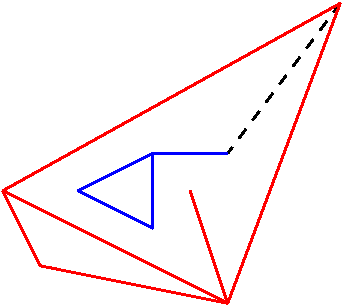
\includegraphics[height=4cm]{img/fig11.pdf}
\sampleEND

\end{document}
